\subsection{Visualization}
To demonstrate the potential applications of Synopsis, we created two representative visualizations. Our first visualization generated a climate chart by issuing statistical queries to retrieve high, low, and mean temperature values as well as precipitation information for a given spatial region. Climate charts are often used to provide a quick overview of the weather for a location; Figure~\ref{fig:climate} summarizes the temperature and precipitation in Snowmass Village, Colorado during 2014. While a standard approach for producing these visualizations over voluminous atmospheric data would likely involve several MapReduce computations, our sketchlets make all the necessary information readily available through queries, avoiding distributed computations altogether.

\begin{figure}
    \centerline{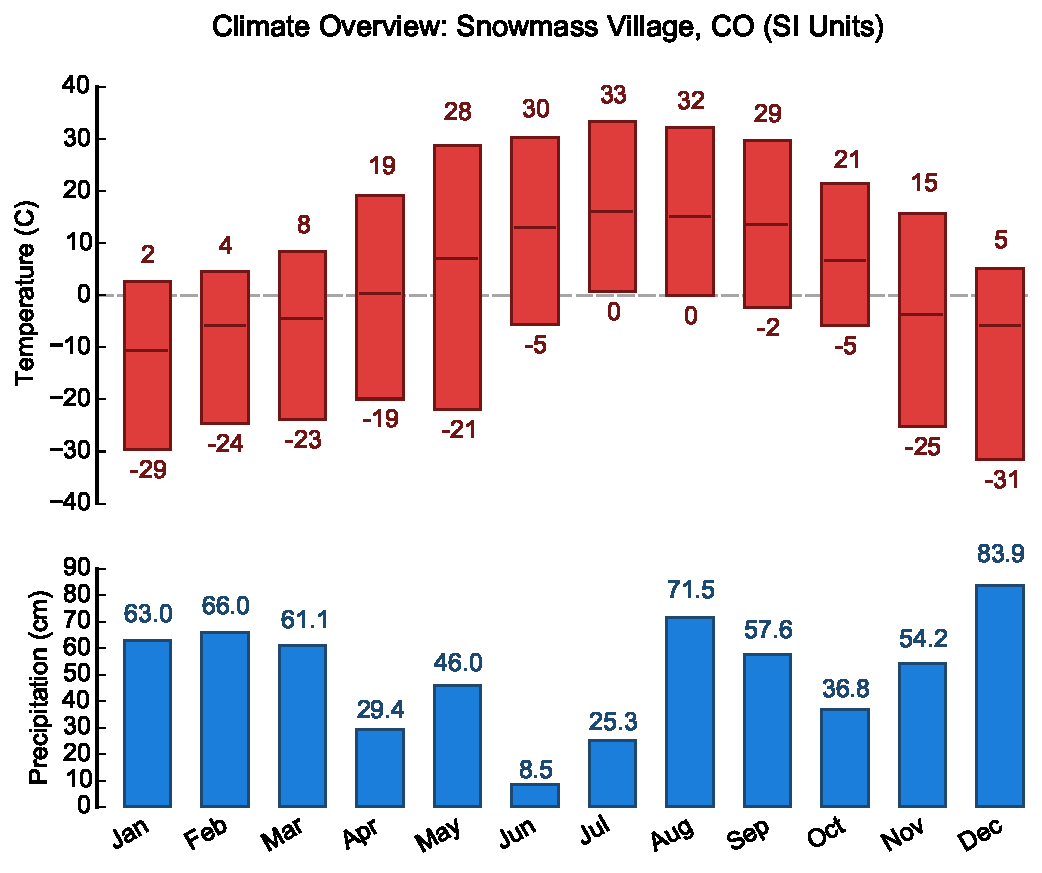
\includegraphics[width=\linewidth]{figures/climate-snowmass.pdf}}
    \caption{Climate chart visualization}
    \label{fig:climate}
\end{figure}

Our second visualization ...

\begin{figure}
    \centerline{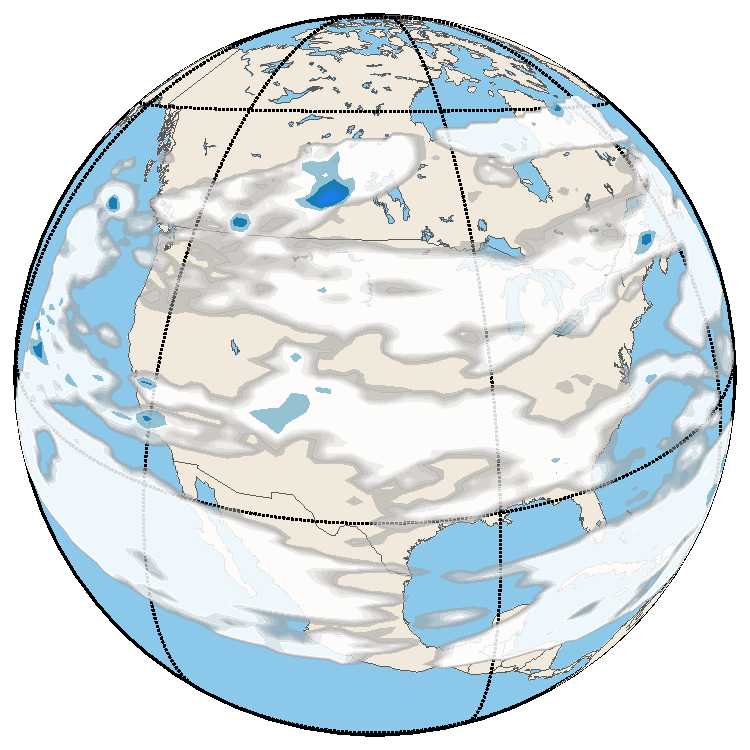
\includegraphics[width=\linewidth]{figures/globe.pdf}}
    \caption{Global contour visualization}
    \label{fig:global-contour}
\end{figure}


